\begin{frame}
\frametitle{Preprocesamiento para SVM}

\begin{itemize}
	\item Eliminación de variables. 
	\begin{itemize}
		\item $region$, $recorded\_by$, $num\_private$,...
		\item Variables categóricas con más de 100 valores.
	\end{itemize}
	\pause
	\item Detección de valores perdidos(NA).
	\begin{itemize}
		\item $population = 0$??
		\item $construction\_year = 0$??
		\item Valores vacios.
	\end{itemize}
	\pause
	\item Cambiar tipos de dato.
	\begin{itemize}
		\item $region\_code$/$district\_code$ a factor.
		\item $date$ a numérico.
	\end{itemize}
\end{itemize}



\end{frame}

\begin{frame}

\frametitle{Limpieza de ruido mediante IPF}

	
	\begin{exampleblock}{IPF(Iterative partitioning filter)}
	
		\begin{itemize}
			\item Split the current training dataset E into $n$ equal sized subsets.
			\item  Build a classifier with the C4.5 algorithm over each of these $n$ subsets and use them to evaluate the whole current training dataset E.
			\item Add to A the noisy examples identified in E using a voting scheme (consensus or majority).
			\item Remove the noisy examples.
			
		\end{itemize}
		Sáez, J. A., Luengo, J., Stefanowski, J.,  Herrera, F. (2015). SMOTE–IPF: Addressing the noisy and borderline examples problem in imbalanced classification by a re-sampling method with filtering. Information Sciences, 291, 184-203.
	\end{exampleblock}

	


\end{frame}

\begin{frame}

\frametitle{Imputación de valores perdidos}

\begin{itemize}
	\item Amelia para valores perdidos numéricos(método iterativo de imputación).
	
	\item Imputación mediante KNN de valores categóricos(moda).
	
\end{itemize}

\end{frame}


\begin{frame}
\frametitle{Duminicación de variables}

\begin{itemize}
	\item Para cada valor las variables categórica, creamos una variable que valdrá 1 si la instancia tiene este valor.
	\item Eliminamos una de las variables dumificadas ya que no aporta más información.
\end{itemize}

\end{frame}

\begin{frame}
\frametitle{PCA para variables dumificadas. Selección de subespacios relevantes}

\begin{itemize}
	\item Normalizamos las variables para aplicar PCA.
	\item Aplicamos PCA y nos quedamos con las variables cuya desviación típica sea mayor de un umbral(0.00001).
	\item Pasamos de 208 variables a 132.
\end{itemize}
\end{frame}

\begin{frame}
\frametitle{Aplicación de SMOTE para balancear clases}

El método SMOTE genera instancias de la clase minoritaria, sobrerepresentandola. Mejora la clasificación de instancias minoritarias pero no la tasa de acierto.

\end{frame}

\begin{frame}
\frametitle{Flujo de información}
\begin{figure}
	\centering
	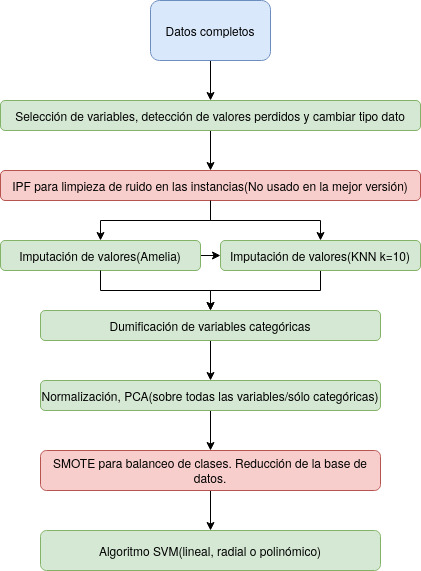
\includegraphics[width=0.5\linewidth]{figures/DiagramaFlujoSVM}
	\caption{Verde: Utilizado en el mejor modelo}
	\label{fig:diagramaflujosvm}
\end{figure}


\end{frame}


\begin{frame}
\frametitle{Puntuación a lo largo del tiempo de SVM}

\begin{figure}
	\centering
	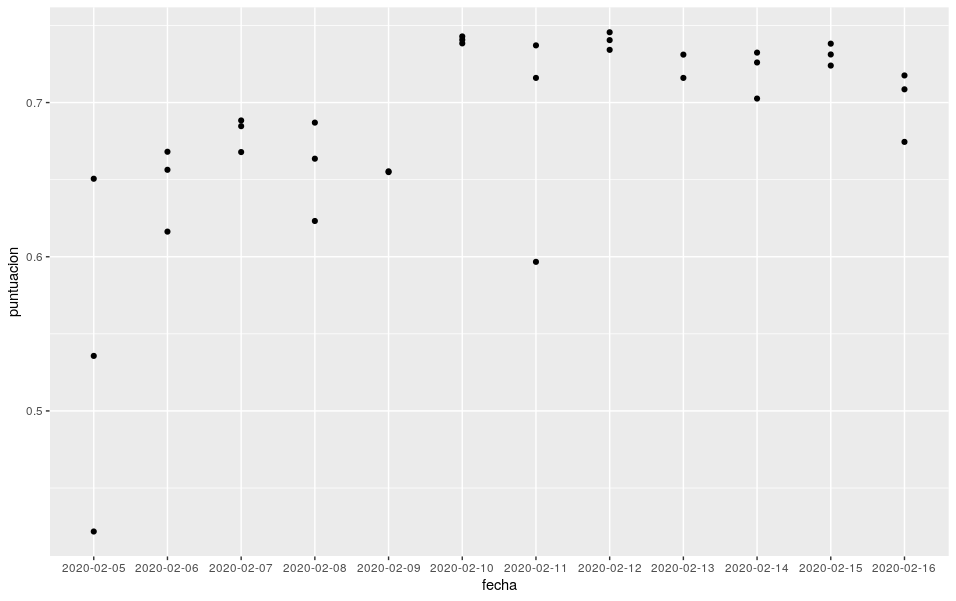
\includegraphics[width=\linewidth]{figures/puntuacionSVM}
	\caption{Máxima puntuación: 74.52\% el 12 de febrero}
	\label{fig:puntuacionsvm}
\end{figure}


\end{frame}